\chapter*{Introduction}
\label{cap:introduction}
\addcontentsline{toc}{chapter}{Introduction}

Introduction to the subject area. This chapter contains the translation of Chapter \ref{cap:introduccion}.

Nowadays, due to the large number of video game users in different regions, there arises a need to adapt video games to countries or regions different from where they were originally developed. For this purpose, there is a series of steps or strategies that can be followed. In this work, I will design a tool to assist in this process.

\section{Motivation}
Over the years, video games have become one of the largest entertainment industries in the world. According to a report by \cite{NZIngreso2024}, in 2024 the global video game market reached an estimated revenue of 187.7 billion dollars, as shown in Figure \ref{fig:NewZooRevenues_E}. The same report shows the growth in the number of players (Figure \ref{fig:NewzooPlayers_E}), from 3.14 billion in 2022 to 3.422 billion in 2024, with a prediction of 3.759 billion by 2027.

\begin{figure}[H]
	\centering
	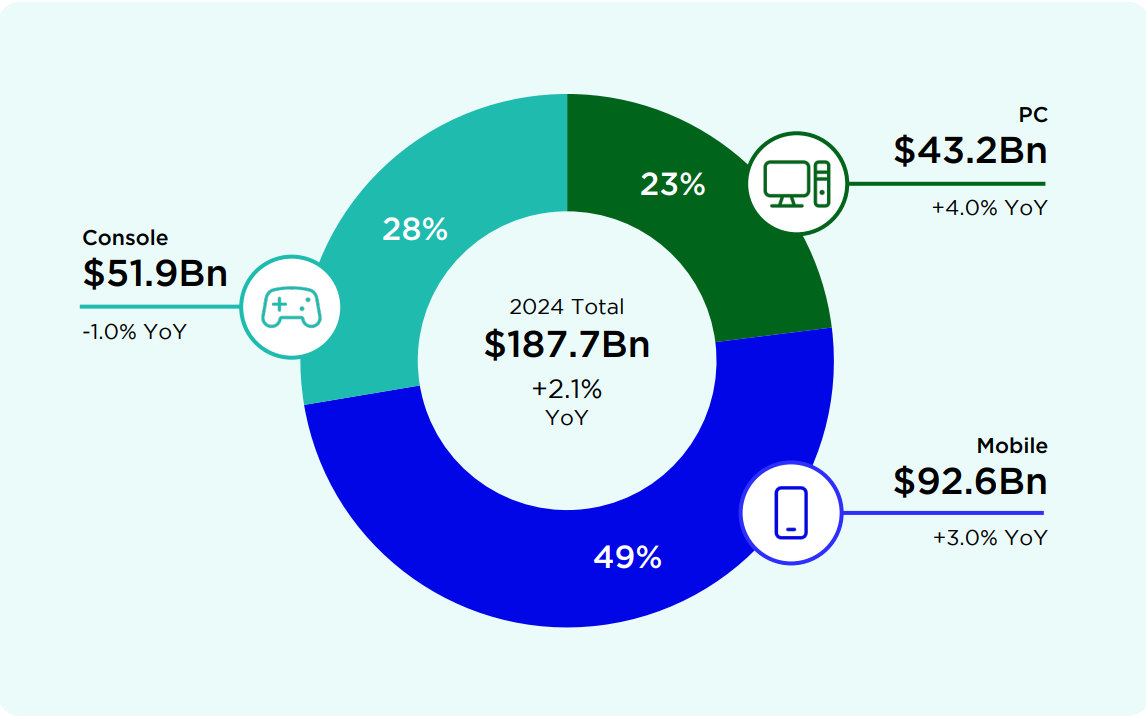
\includegraphics[width = 0.5\textwidth]{Imagenes/Newzoo_2024_Revenues.png}
	\caption{Estimated revenue in the video game industry in 2024. Newzoo}
	\label{fig:NewZooRevenues_E}
\end{figure}

\begin{figure}[H]
	\centering
	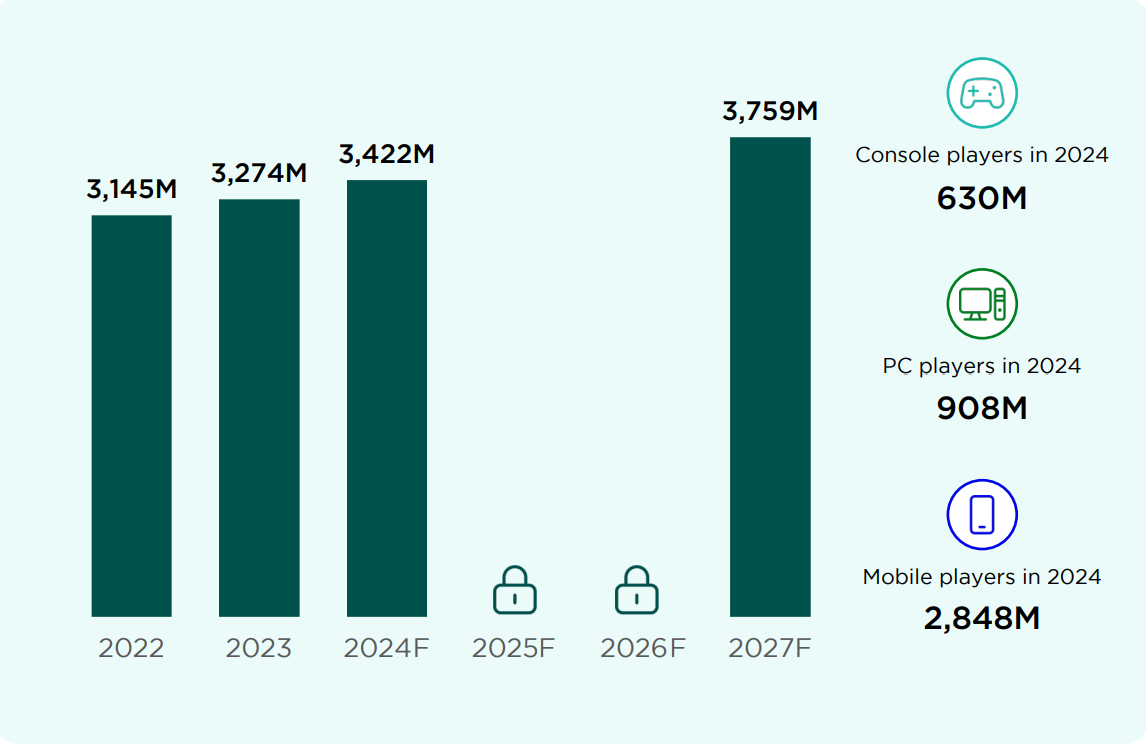
\includegraphics[width = 0.5\textwidth]{Imagenes/Newzoo_Players.png}
	\caption{Global players 2022–2024 and projection for 2027. Newzoo}
	\label{fig:NewzooPlayers_E}
\end{figure}

Additionally, the same report mentions the percentage of players by region, with the Asia-Pacific region representing more than half (53\%) of global players, as shown in Figure \ref{fig:NewzooPlayersReg_E}.  
Given this growth and these figures, there is a need to adapt video games to different languages and cultures through the processes of internationalization ({\textit{I18N}}) and localization ({\textit{L10N}}), in order to be published in various regions and countries.

\begin{figure}[H]
	\centering
	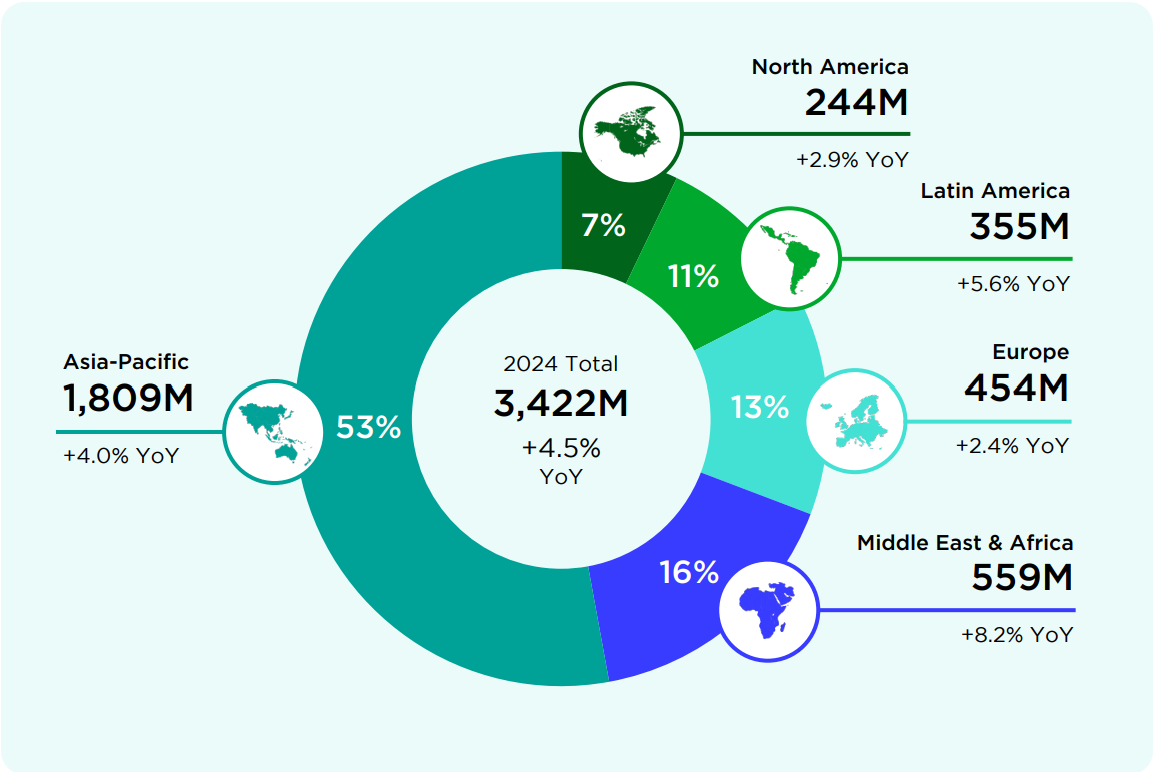
\includegraphics[width = 0.5\textwidth]{Imagenes/Newzoo_Players_Region.png}
	\caption{Percentage of players by region. Newzoo}
	\label{fig:NewzooPlayersReg_E}
\end{figure}

Internationalization is the process by which a video game is prepared from its early development stages to support different cultures and languages, so that no major modifications to the code are needed later.  
On the other hand, localization is the process of translating and adapting the texts, graphics, and resources of a video game to the various cultures in which it will be released.

During both of these processes, various types of errors may occur (such as translation or display errors). This is where \textit{Localization Quality Assurance} (LQA) comes into play. This process involves reviewing and testing different parts of the game to ensure that none of these errors occur and that the final product is appropriate for the target culture and audience.

Until now, this process has been carried out manually, where testers meticulously check each piece of text and how it is displayed within the game, which requires a significant amount of time and resources. While there are tools to automatically check the correctness of translations and texts, the same cannot be said for verifying how texts are displayed within the context of the game.

Based on the points discussed above, our motivation for this work is to automate testing of internationalization and localization processes in order to save time and resources, which can then be redirected to other more critical areas.  
To achieve this, we will use computer vision techniques and \textit{Optical Character Recognition} (OCR) so that, given a screenshot of a video game, we can extract the text and perform various checks and tests on it.

\section{Objectives}
The main objective of this project is the design and implementation of a tool to assist in the automation of localization QA.  
To achieve this main goal, the following secondary objectives are proposed:

\begin{enumerate}
	\item Research the LQA process and the tools used, as well as the most common errors in internationalization and localization.
	\item Investigate OCR technologies and how to use them, in order to choose one that fits our requirements by conducting tests and comparisons.
	\item Design a series of OCR-based automated tests to detect common linguistic errors.
	\item Deploy the tool using a Docker image so that it can be run on any machine.
	\item Integrate the OCR to use its output as input for the tests, and improve the OCR's accuracy as much as possible.
	\item Evaluate our tool to ensure it produces an acceptable accuracy rate.
\end{enumerate}

\section{Work Plan}
To achieve our objectives, we will follow the steps below:

\begin{enumerate}
	\item Research and understand the processes of internationalization, localization, and LQA, as well as the most common linguistic errors that occur during video game development (Chapter \ref{cap:estadoDeLaCuestion}).
	\item Select the most common localization errors that are related to character or positioning issues and that can be detected using OCR (Chapter \ref{cap:descripcionTrabajo}).
	\item Develop a series of tests capable of detecting specific localization errors using OCR-generated data as input (Chapter \ref{cap:implementacion}).
	\item Investigate different OCRs, understand how they work, how to use them to detect text in images, and how to train a model knowing the language and font used (Section \ref{sec:Seleccion de libreria de OCR}).
	\item Evaluate the selected OCRs based on performance and accuracy. Explore methods to increase accuracy (Chapter \ref{cap:evaluacion}).
	\item Perform separate evaluations of each module (OCR and testing) (Chapter \ref{cap:evaluacion}).
	\item Integrate both modules and conduct a comprehensive evaluation of the entire tool (Chapter \ref{cap:evaluacion}).
	\item Generate output that is easily interpretable by humans (Section \ref{sec:Generación informe}).
\end{enumerate}








